Conventional topological insulators (\hypertarget{TI}{TI})~\cite{FuKaneMele3D,Roy07,MooreBalents07,QiHughesZhang08} are time reversal and charge $U(1)$ symmetric electronic band insulators in three dimensions that host massless surface Dirac fermions. The topologically protected surface Dirac fermion can acquire a single-body ferromagnetic or superconducting mass by breaking time reversal or charge $U(1)$ symmetry respectively, as described in the introduction chapter. Alternatively it can acquire a many-body interacting mass while preserving both symmetries, and exhibit long-ranged entangled surface topological order~\cite{WangPotterSenthilgapTI13,MetlitskiKaneFisher13b,ChenFidkowskiVishwanath14,BondersonNayakQi13}. Interfaces between different massive surface domains host exotic massless quasi-$(1+1)$D electronic channels~\cite{TeoKane,FuKanechargetransport09,QiWittenZhang13}, and consequently, from the bulk-boundary correspondence, topological insulator slabs with distinct gapped surface orders lead to a variety of quasi-$(2+1)$D topological phases. 
On the other hand, fractional topological insulators (\hypertarget{FTI}{FTI})~\cite{MaciejkoQiKarchZhang10,SwingleBarkeshliMcGreevySenthil11,maciejko2012models,ye2016composite,maciejko2015fractionalized,stern2016fractional,YeChengFradkin17} are long-range entangled topologically ordered electronic phases in $(3+1)$ dimensions outside of the single-body mean-field band theory description. They carry fractional quasi-particle and quasi-string excitations that cannot be adiabatically connected to the electron. 
They carry time reversal and charge $U(1)$ symmetries, which enrich its topological order (local excitation spectrum) in the sense that a symmetric surface must be anomalous and cannot be realized non-holographically by a true $(2+1)$-D system. In this paper, we describe the topological properties of various massive surface states and quasi-$(2+1)$-D slabs of a series of a fractional topological insulator. In particular, we focus on the quasi-particle structure.

\begin{figure}[htbp]
\centering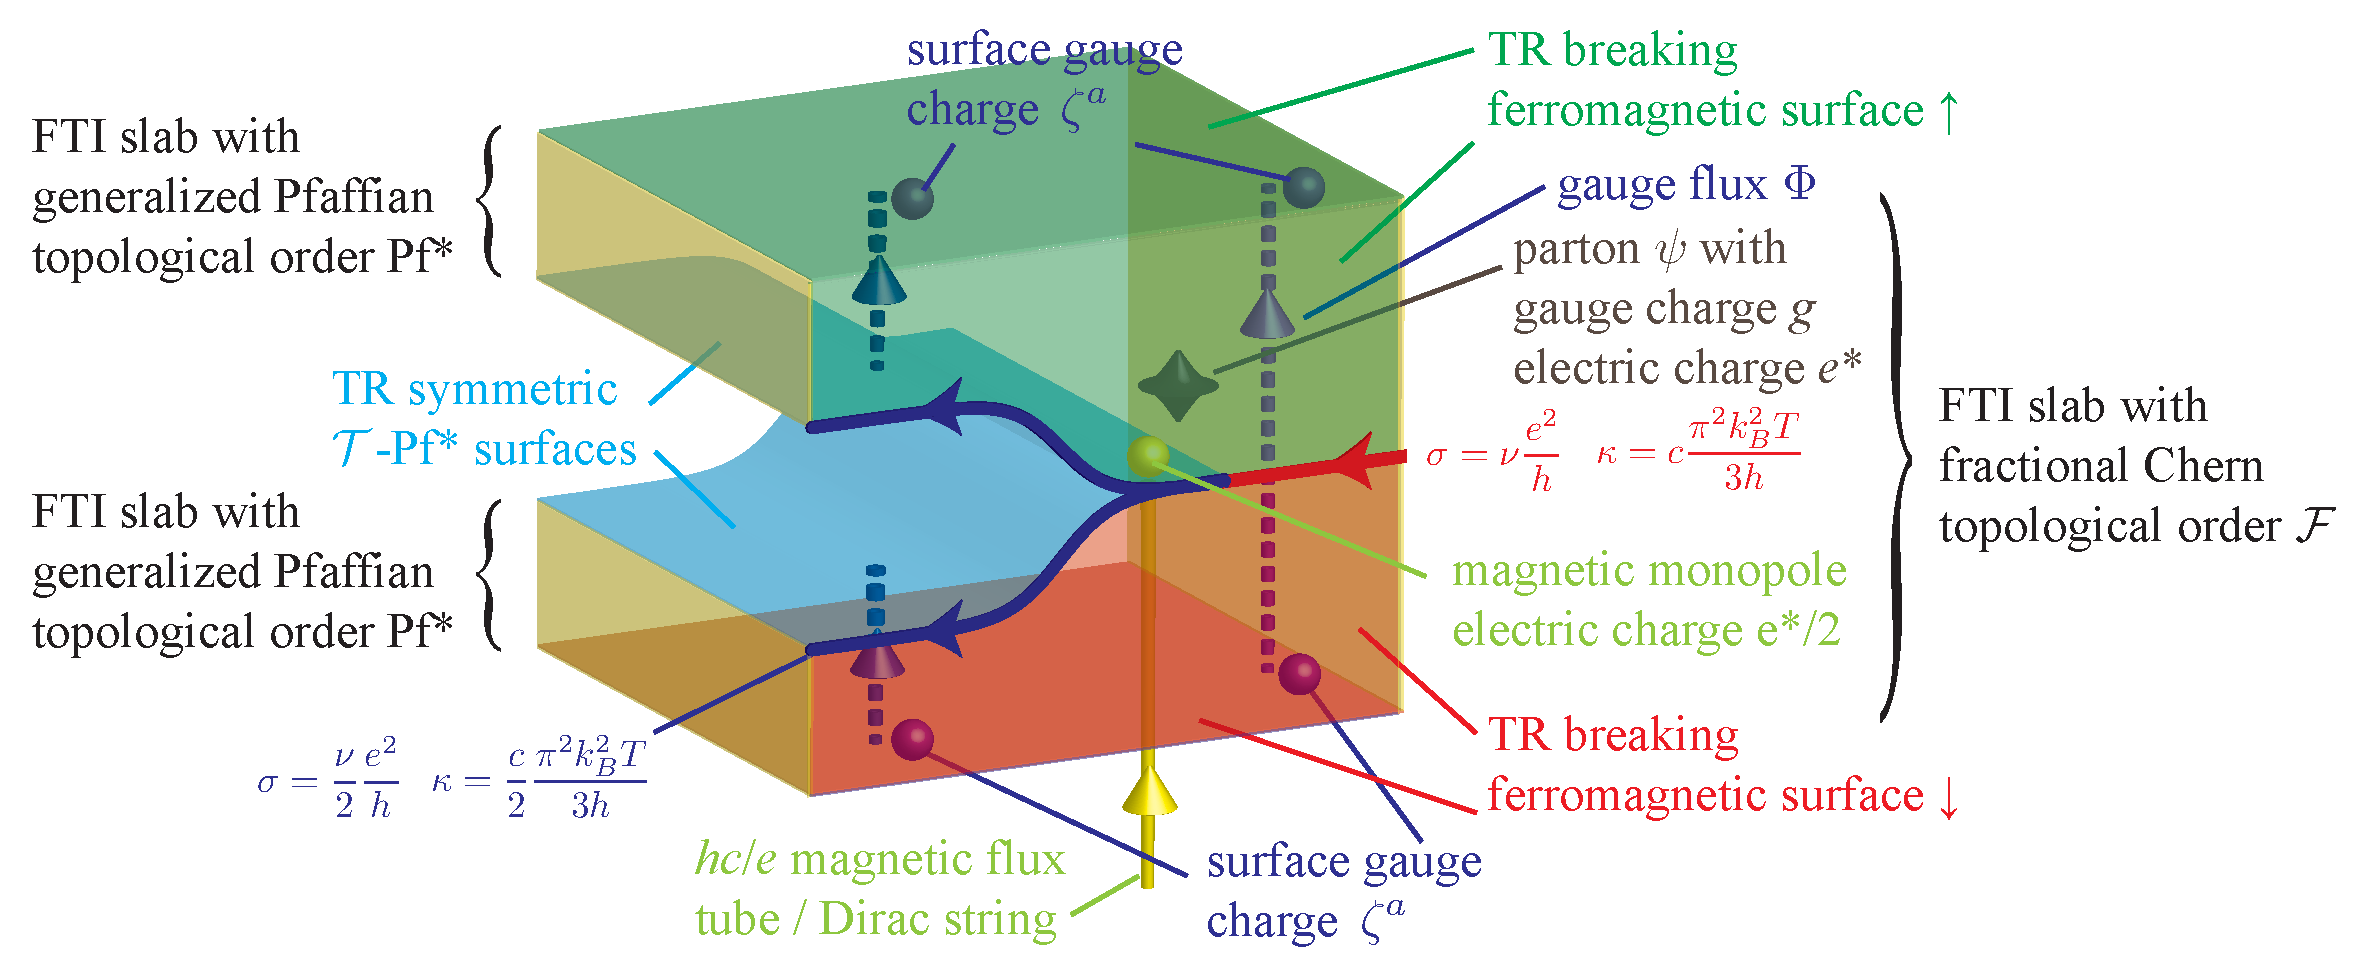
\includegraphics[width=0.9\textwidth]{fig1}
%\caption{Summary of the \QP and gauge flux content in \FTI slabs. A pair of $\mathrm{Pf}^\ast$ \FTI slabs are merged into a fracional Chern \FTI slab $\mathcal{F}$ by gluing the two \TR symmetric \TPf surfaces. Directed bold lines on the front surfaces are chiral edge modes of the $\mathrm{Pf}^\ast$ and $\mathcal{F}$ \FTI slabs.}\label{fig1}
\caption{Summary of the quasiparticle and gauge flux content in fractional topological insulator slabs. A pair of $\mathrm{Pf}^\ast$ fractional topological insulator slabs are merged into a fractional Chern insulator slab $\mathcal{F}$ by gluing the two time reversal symmetric $\mathcal{T}$-$\mathrm{Pf}^\ast$ surfaces. Directed bold lines on the front surface are chiral edge modes of the $\mathrm{Pf}^\ast$ and $\mathcal{F}$ fractional topological insulator slabs.}\label{fig1}
\end{figure}

We focus on a series of fermionic fractional topological insulators, labeled by integers $n$, whose magneto-electric response is characterized by the $\theta$-angle $\theta=\pi/(2n+1)$ (modulo $2\pi/(2n+1)$) that associates an electric charge of $e^\ast/2=e/2(2n+1)$ to each magnetic monopole~\cite{Witten79}, for $e$ the electric charge of the electron. In particular, we consider fractional topological insulators that support deconfined fermionic parton excitations $\psi$ in the bulk, each carrying a fractional electric charge of $e^\ast=e/(2n+1)$. This assumes the electron can be written as 2n+1 parts, i.e.  $\psi_{\mathrm{el}}\sim\psi_1\ldots\psi_{2n+1}$. The $(3+1)$-D topological order is based on a discrete $\mathbb{Z}_{2n+1}$ gauge theory~\cite{maciejko2012models}. This is necessary because these particles do not exist outside of the insulator, and so must glue together. This gauge theory ensures that, and there are several ways to do this but we just consider one.  The theory supports electrically neutral string-like gauge flux $\Phi$, so that a monodromy quantum phase of $e^{2\pi ig/(2n+1)}$ is obtained each time $\psi$ orbits around it. In other words, $\psi$ carries the gauge charge $g$ that braids with the gauge flux. The integer $g$ and $2n+1$ are relatively prime so that all local quasiparticles be combinations of the electronic quasiparticles $\psi_{\mathrm{el}}$ and hence must carry integral electric charges and trivial gauge charges.

Generalizing the surface state of a conventional topological insulator, the surface of a fractional topological insulator hosts massless Dirac partons coupling with a $\mathbb{Z}_{2n+1}$ gauge theory. These anyons are bosons. Unlike its non-interacting counterpart whose gapless Dirac surface state is symmetry protected in the single-body picture, a fractional topological insulator is strongly interacting to begin with and there is no topological reason for its surface state to remain gapless. In this paper we focus on three types of gapped surface states -- ferromagnetic surfaces that break time reversal, superconducting surfaces that break charge $U(1)$, and symmetric surfaces which generalize the $\mathcal{T}$-Pfaffian surface state of a conventional topological insulator and is denoted by {$\mathcal{T}$-$\mathrm{Pf}^\ast$}. The topological order for fractional topological insulator slab with these surfaces are discussed in Sec.~\ref{FS}, \ref{SCS} and \ref{TPF} respectively. In Sec.~\ref{Gluing}, we discuss, using an anyon condensation picture, the gluing of a pair of $\mathcal{T}$-Pfaffian surfaces. We conclude in Sec.~\ref{Conclusion} with remarks on a complementary way to understand these topological order \cite{ChoTeoFradkin17}.